\documentclass[a4paper,12pt]{article}

\usepackage[fleqn]{amsmath}
\usepackage{amssymb}
\usepackage{fancyhdr}
\usepackage{geometry}
\usepackage{enumerate}
\usepackage{graphicx}
\usepackage{hyperref}
\usepackage{geometry}
\usepackage{verbatim}

\usepackage{alltt}                                
\usepackage{float}
\usepackage{color}
\usepackage{url}
\usepackage{multicol}
\usepackage{balance}
\usepackage[TABBOTCAP, tight]{subfigure}
\usepackage{enumitem}
\usepackage{pstricks, pst-node}

\usepackage{listings}

\geometry{left=2.5cm,right=2.5cm,top=3cm,bottom=2.5cm}
\setlength{\parskip}{0.5\baselineskip}
\lstset{language=Python} 
\begin{document}
\setlength\parskip{ \baselineskip}
\title{Project \#2 : OpenMP: N-body Problem -- Coarse vs Fine and Static vs Dynamic}
\setlength\parskip{ \baselineskip}
\author{
	Huan Yan
}

\maketitle
\newpage
\renewcommand{\headrulewidth}{1pt}
\renewcommand{\labelitemii}{$\bullet$}
\def\course{CS575}
\def\name{Huan Yan}

\parindent = 0.0 in
\parskip = 0.1 in


\hfill \course


\hfill \name


\hfill \today

\subsection*{ 1. Tell what machine you ran this on}

For project2, I compiled and ran the code on flip.engr.oregonstate.edu.  And use the command lscpu that we can see the information about the CPU as follows:\\

\includegraphics[width=6in]{1}

\subsection*{2. Create a table with your results.}

In this project, I use \textbf{400 bodies}, and \textbf{300 time steps}.\\

I use the \textbf{Threads are from 1 to 64}.\\

We can get the answer from the following table:\\

\begin{tabular}{|l|l|l|l|l|}
\hline
\textbf{\# of threads} & \textbf{Coase + Static} & \textbf{Coase + Dynamic} & \textbf{Fine + Static} & \textbf{Fine + Dynamic} \\ \hline
1                      & 17.732261             & 16.843331              & 17.056532            & 10.871653             \\ \hline
2                      & 35.260576             & 34.815725              & 29.70031             & 8.285783              \\ \hline
4                      & 63.895304             & 65.447648              & 42.411583            & 11.476287             \\ \hline
8                      & 90.004253             & 101.960867             & 37.600903            & 12.851895             \\ \hline
16                     & 155.113356            & 154.669451             & 32.884484            & 0.471237              \\ \hline
24                     & 31.664904             & 33.528267              & 0.069595             & 0.043506              \\ \hline
32                     & 104.779648            & 134.065597             & 2.819759             & 2.437727              \\ \hline
64                     & 84.057365             & 122.922764             & 1.548711             & 1.448382              \\ \hline
\end{tabular}


\subsection*{3. Draw a graph. }

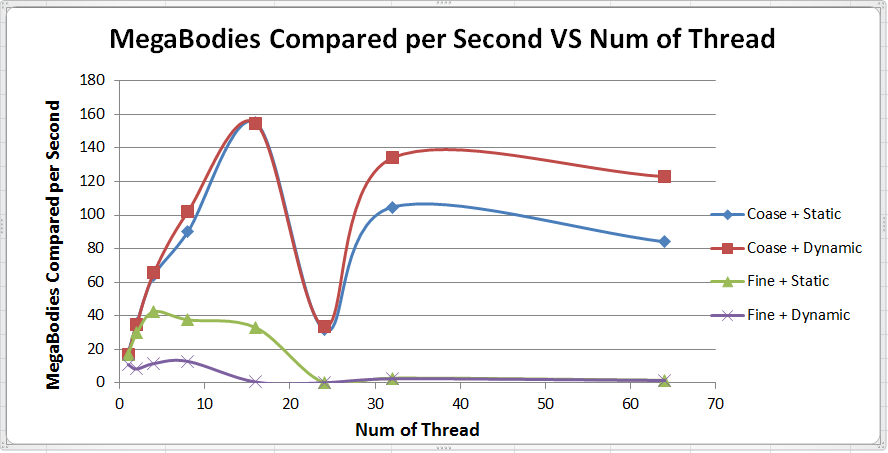
\includegraphics[width=6in]{3}

\subsection*{4. What patterns are you seeing in the speeds?}

In Figure, the two curves of coarse-grained parallelism are above the curves of fine-grained parallelism mostly.

With the increasing of threads amount, curves of coarse-grained parallelism go up firstly until around 16-thread. Then, they go down sharply until around 24-thread. And they go up again until around 32-thread. Finally, curves of coarse-grained parallelism go down. Especially, coarse+static curve spend less mega bodies than coarse+dynamic curve after 24-thread.

For curves of fine-grained parallelism, when number of thread is going up, they go down at first until around 24-thread. Specially, curve of fine+static is above curve of fine+dynamic, and slopes down faster than curve of fine+dynamic.

\subsection*{5. Why do you think it is behaving this way?}

From Figure, intuitively, coarse-grained parallelism performs better than fine-grained parallelism. Coarse-grained parallelism allows a single thread occupying resource as much as possible firstly. If this single thread takes too long time to response, then the resource will be given to next thread. Fine-grained parallelism will fairly provide resource to each thread. In this case, since fine-grained parallelism switches among threads more frequently than coarse-grained parallelism, it cannot gain lots of mega bodies per a second. Thus, the curves of coarse-grained parallelism are above the curves of fine-grained parallelism mostly.

Also, for picture, because the CPU contains 24 cores, when number of threads increase to 24, CPU reaches to the limitation of physical machine. And then, when system applies for more number of threads, virtual threads will be arranged to support work. Performance of virtual thread is not as good as physical thread. Thus, the curves of coarse-grained parallelism after 24-thread cannot reach to the same level with the part of curve before 24-thread.

By comparing the curves between static thread and dynamic thread, we can see that there is no obvious regulation. I think static thread allocate and assign work at runtime. The curve trend of static thread in figure is more stable. Dynamic thread will provide resource according to algorithm. It could affect performance a lot.

\end{document}
